To extend the BONUS results to higher $x$, a proposal~\cite{BONUS12} for 
35~days of running on gaseous deuterium and 5~days on gaseous hydrogen at 
11~GeV was submitted to JLab PAC30 and conditionally approved.  The experiment 
will use the standard {\tt CLAS12} equipment with the additional recoil 
detector already used in E03-012~\cite{BONUS}.  The anticipated results can be 
seen in Fig.~\ref{fig:b12xpctd} for $F_2^n/F_2^p$ (left) and $u/d$ (right). 
Clearly the $F_2^n/F_2^p$ data obtained using the new method will allow us to 
differentiate unambiguously between different expectations for this ratio.

%%%%%%%%%%%%%%%%%%%%%%%%%%%%%%%%%%%%%%%%%%%%%%%%%%%%%%%%%%%%%%%%%%%%%%%%%%%
\begin{figure}[ht!]
\begin{center}
\centerline{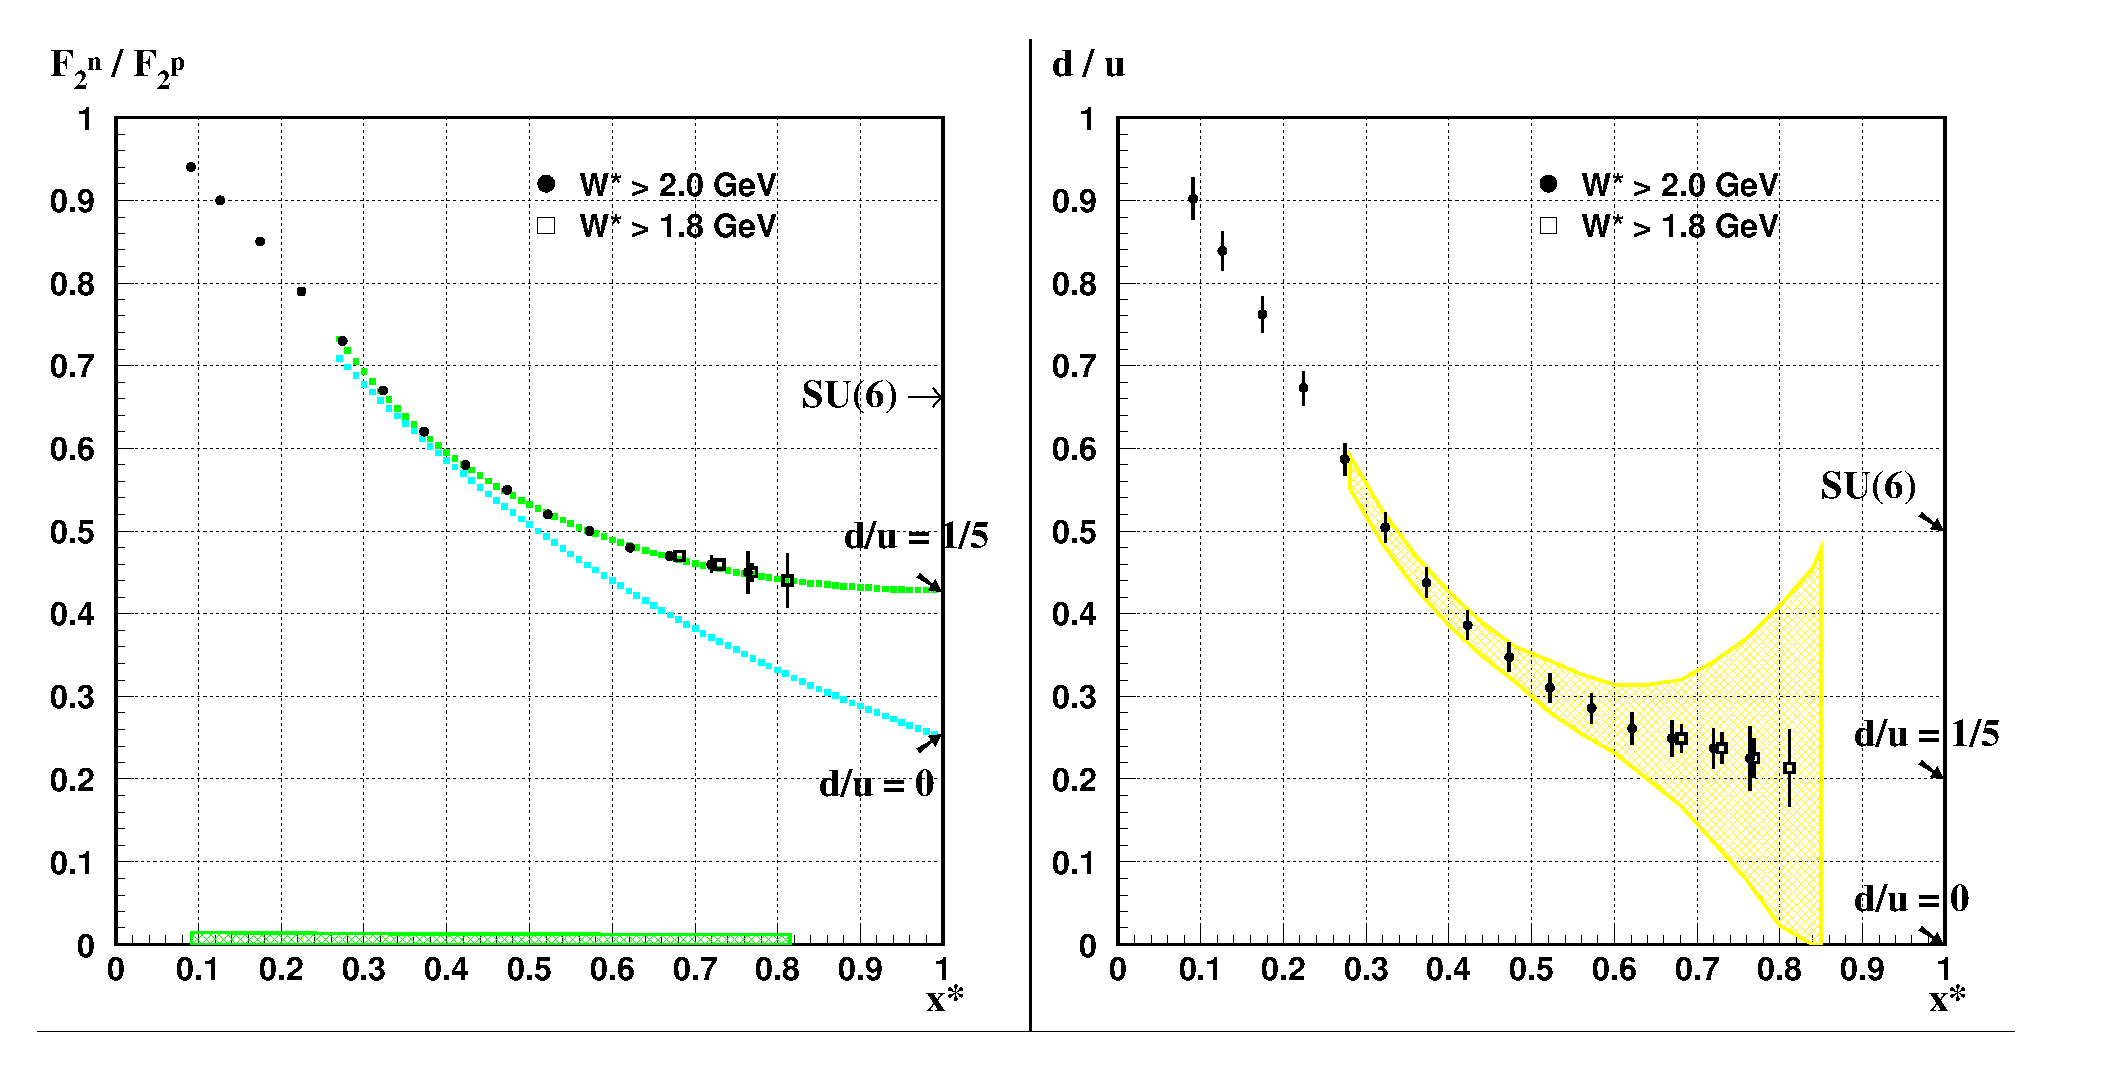
\includegraphics[scale=0.4, angle=0]{../strucfunc/bonus_12_xpctd.eps}}
\end{center}
\vspace*{-1cm}
\caption{\small{Anticipated results on $F_2^n/F_2^p$ (left) and the extracted 
$u/d$ ratio (right) for 40~days of data taking at 11~GeV with {\tt CLAS12}.  
The arrows along the ordinate indicate model predictions.  The error bars 
pertaining to filled circles are statistical with a $W>2$~GeV constraint.  
The smaller errors (with open squares) are for $W>1.8$~GeV.  The systematic 
error is indicated by the band along the abscissa on the left plot.  The two 
curves on the left plot represent hadron-parton duality based predictions 
with two different mechanisms for SU(6) symmetry breaking. The shaded band 
on the right plot indicates our present knowledge on the $d/u$ ratio.}}
\label{fig:b12xpctd}
\end{figure}
%%%%%%%%%%%%%%%%%%%%%%%%%%%%%%%%%%%%%%%%%%%%%%%%%%%%%%%%%%%%%%%%%%%%%%%%%%%

JLab PAC30 also approved E12-06-109 \cite{EG12} which will, in particular,
study polarized parton distributions at large $x$. Using standard detection 
equipment, a redesigned polarized target adapted to {\tt CLAS12} and 30 
(50)~days of running on a longitudinally polarized NH$_3$ (ND$_3$) target, 
high precision measurements can be achieved as shown in Fig.~\ref{fig:A1xpctd}. 
These data will disentangle models in the large-$x$ region.  While the results 
shown in Fig.~\ref{fig:A1xpctd} are with a $W>2$~GeV constraint, hadron-parton 
duality studies (see page \pageref{duality}) will tell us by how much this 
constraint can be relaxed, possibly increasing the $x$ range up to 0.9.  The 
expected accuracy for $(\Delta d+ \Delta\bar{d})/(d+\bar{d})$ is 
shown in Fig.~\ref{fig:ddodxpctd}.
 
%%%%%%%%%%%%%%%%%%%%%%%%%%%%%%%%%%%%%%%%%%%%%%%%%%%%%%%%%%%%%%%%%%%%%%%%%%%
\begin{figure}[ht!]
\begin{center}
\centerline{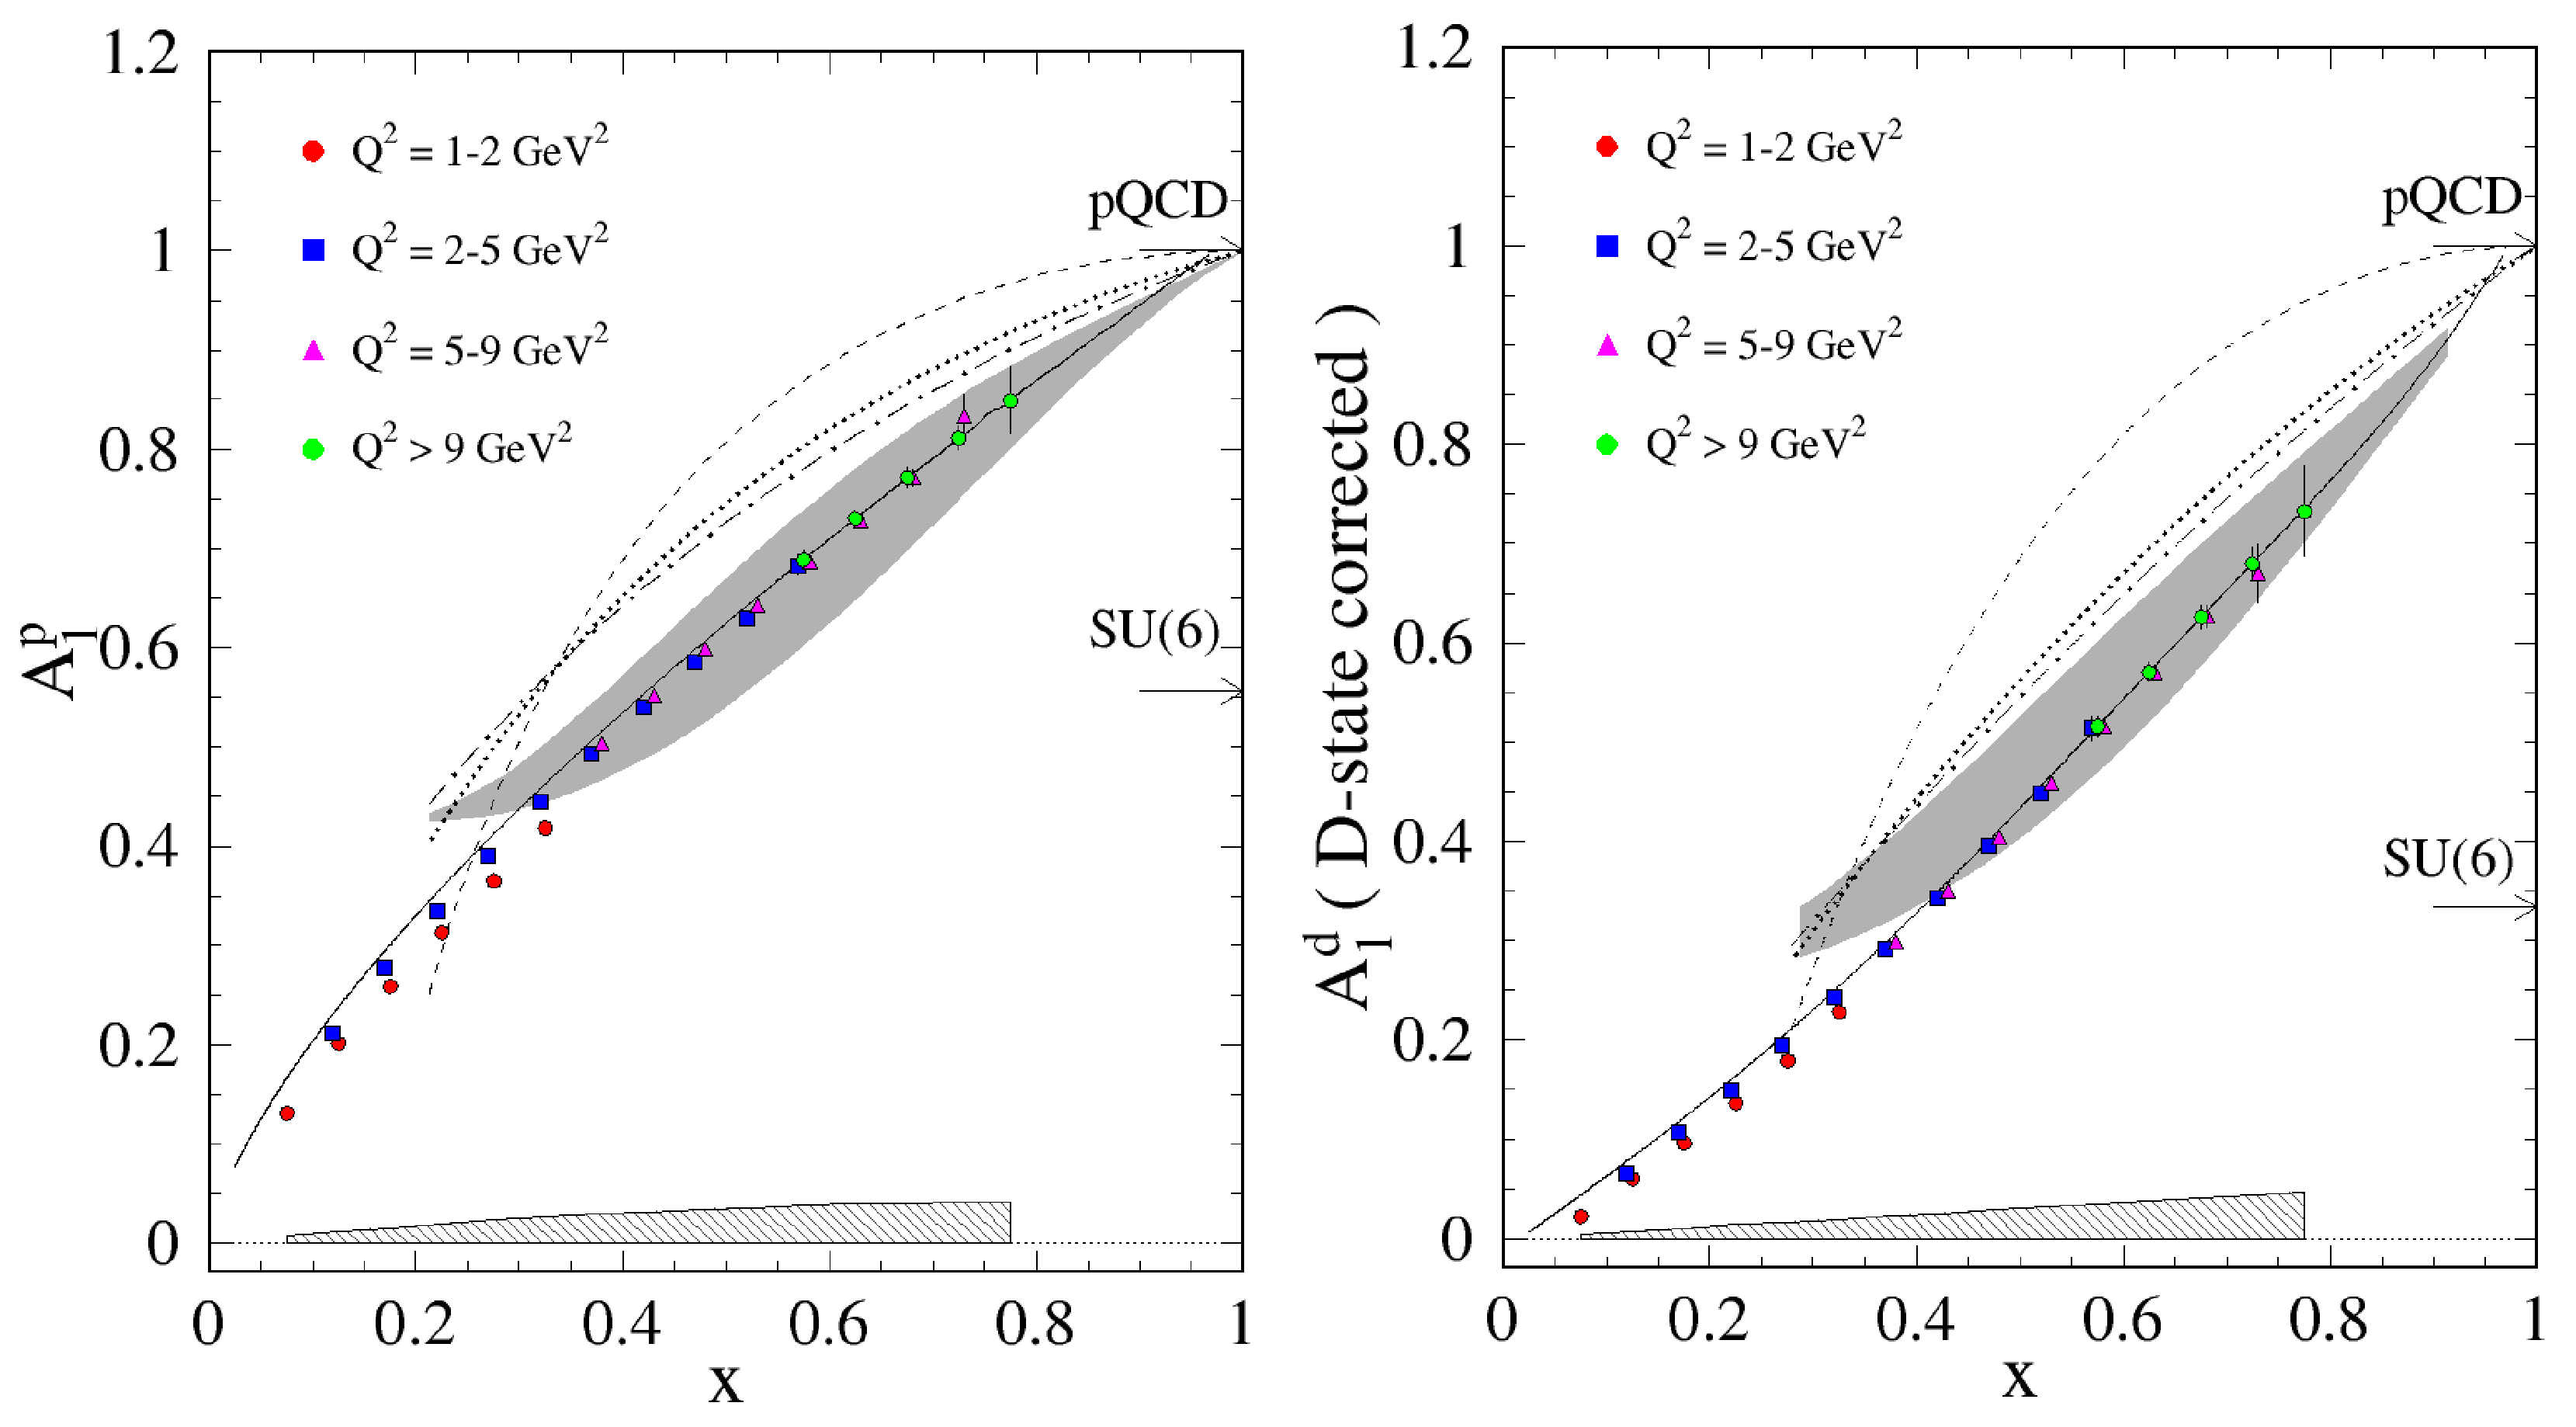
\includegraphics[scale=0.25, angle=0]{../strucfunc/A1_xpctd.eps}}
\end{center}
\vspace*{-1cm}
\caption{\small{Anticipated results on $A_1^p$ (left) and $A_1^d$ (right).
The four different symbols represent four different $Q^2$ ranges.  The 
statistical uncertainty is given by the error bars while the systematic 
uncertainty is given by the shaded band.}}
\label{fig:A1xpctd}
\end{figure}
%%%%%%%%%%%%%%%%%%%%%%%%%%%%%%%%%%%%%%%%%%%%%%%%%%%%%%%%%%%%%%%%%%%%%%%%%%%

%%%%%%%%%%%%%%%%%%%%%%%%%%%%%%%%%%%%%%%%%%%%%%%%%%%%%%%%%%%%%%%%%%%%%%%%%%%
\begin{figure}
\begin{center}
\begin{minipage}[t]{0.55\linewidth}
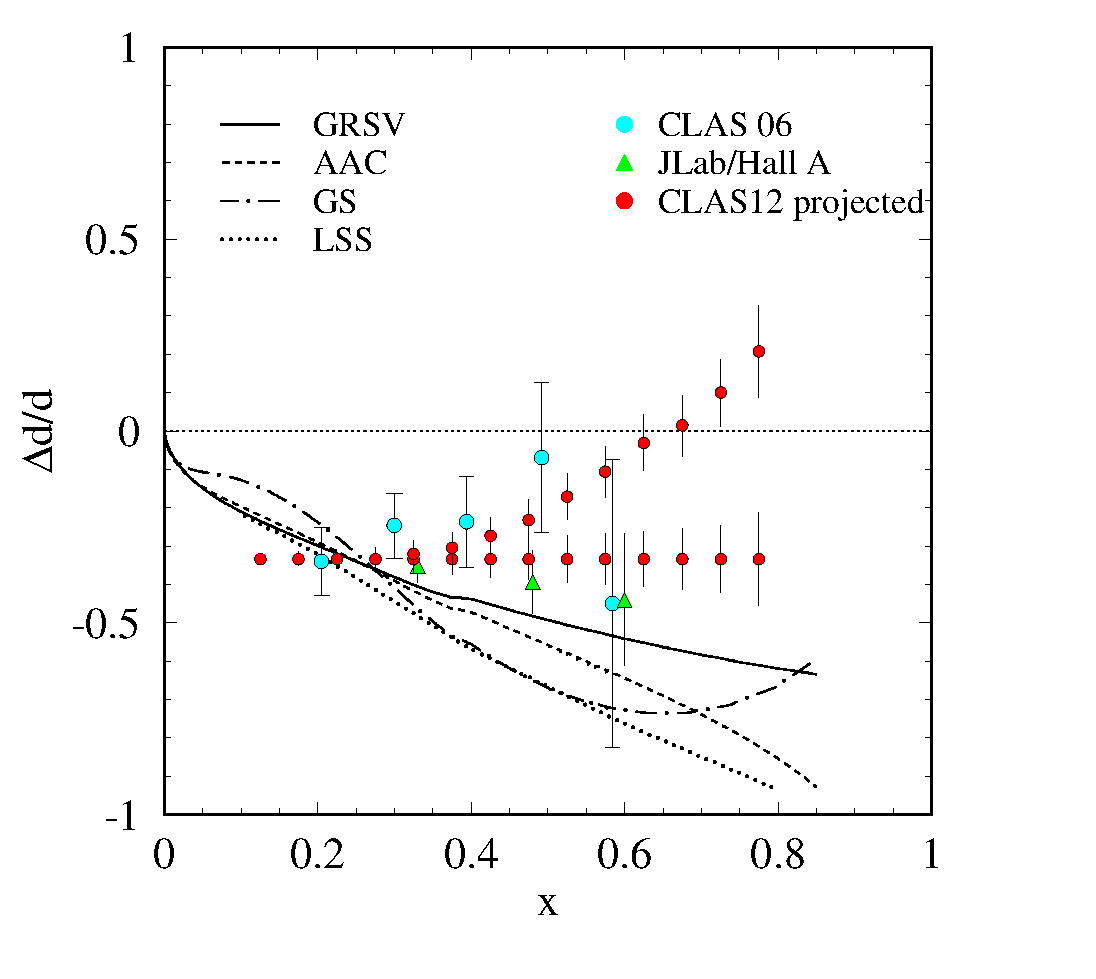
\includegraphics[scale=0.5, angle=0]{../strucfunc/ddod_xpctd.eps}
\end{minipage}\hfill
\begin{minipage}[c]{0.45\linewidth}
\vspace*{-9cm}
\caption{\small{Expected results for $(\Delta d+ \Delta\bar{d})/(d+\bar{d})$. 
The central values of the data are following two arbitrary curves to 
demonstrate how the two categories of predictions, namely the ones that 
predict $\Delta d/d$ stays negative (LO and NLO analyses of polarized 
DIS data: GRSV, LSS, AAC, GS, statistical model, and a quark-hadron duality 
scenario) and the ones predicting $\Delta d/d \to 1$ when $x \to 1$ (leading 
order pQCD and a quark-hadron duality scenario).}}
\label{fig:ddodxpctd}
\end{minipage}
\end{center}
\end{figure}
%%%%%%%%%%%%%%%%%%%%%%%%%%%%%%%%%%%%%%%%%%%%%%%%%%%%%%%%%%%%%%%%%%%%%%%%%%%

